\begin{frame}{B-Splines model}
	\begin{center}
			\begin{minipage}{0.95\textwidth}
			\centering
			\begin{itemize}	
				\item[GOAL] Find optimal transformation $T: (x,y,z) \longmapsto (x', y', z')$
				\item[ALGO]	Spline-based Free-Form Deformation (FFD) : 3D deformation model	using net of points $\phi_{x,y,z}$
			\end{itemize}
		\end{minipage}
		\begin{equation}
	\mathnormal{
		T(x,y,z) = \newline
		\sum _{l=0}^{3}\sum _{m=0}^{3}\sum _{n=0}^{3}{B}_{l}\left(u\right){B}_{m}\left(v\right){B}_{n}\left(w\right){\phi }_{i+l,j+m,k+n}
	}
	\end{equation}
	
	\begin{columns}
		\column{0.4\textwidth}
			Tensor product $\implies$ Calculation by Tensor Cores possible
			
			Each point affects is 4 direct neighbours
		\column{0.6\textwidth}
		\begin{figure}
			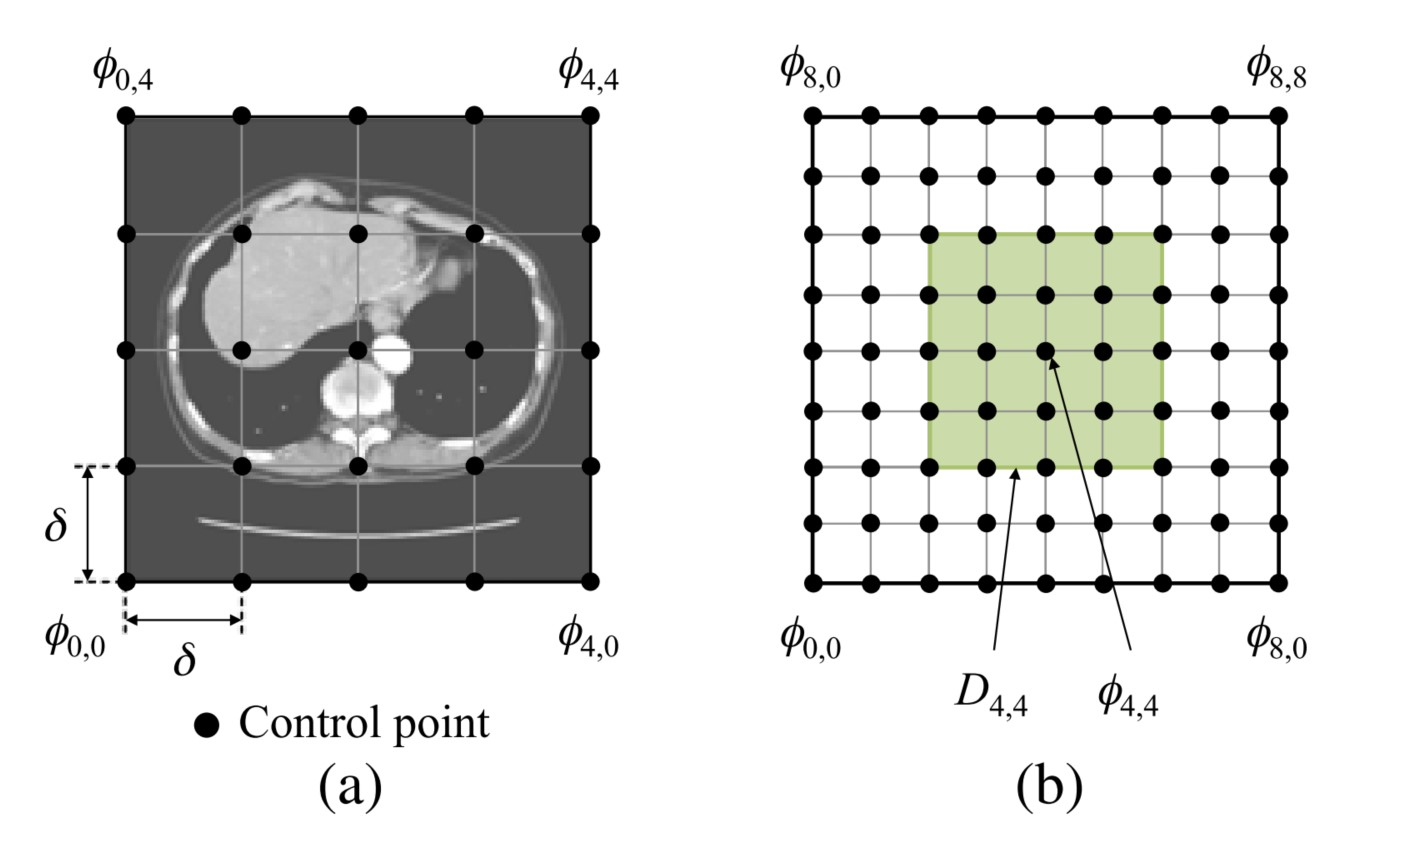
\includegraphics[width=\textwidth]{control_net}
		\end{figure}
	\end{columns}
	
	

	
	\end{center}


	
\end{frame}